\chapter{Game Design}

Before we start implementing the game, we should design its individual parts.
An overall design was described in section~\ref{sec:original-vision}.
In this chapter, we will go into more detail and flesh out the design.
We need to decide which mechanics will be in the game and how will the player interact with them.
The game needs to react to the player's actions and communicate the information the player should know.
This all depends on what exactly are we trying to achieve.
Thus, we will start by setting some design goals.

\section{Design goals}

We aim to make the game's mechanics clear, and controls intuitive and responsive.
This is a necessity for every game because without this, the players can't even properly play the game we want them to play.
This is an important goal that will inform many of our decisions throughout the design.

We have analyzed several games of similar genres to our game, that we find enjoyable, and we tried to identify what makes them fun.
We identified five features, which we think make the games very intriguing and replayable, that we think would work for our game too.
Thus, we intend to design the game, so it exhibits these features, making them our game-specific design goals.
We will explain each in a separate subsection, and we will use other games as inspiration for how to reach them.
The goals are:
\begin{enumerate}
    \item \nameref{sec:goal-depth-battle}
    \item \nameref{sec:goal-depth-run}
    \item \nameref{sec:goal-various-builds}
    \item \nameref{sec:goal-force-exploration}
    \item \nameref{sec:goal-challenge}
\end{enumerate}

\subsection{Strategic Depth in Every Battle} \label{sec:goal-depth-battle}

One of the design goals we identified is that the game should let the player make meaningful strategic decisions throughout every battle.
Each battle should be different enough to require the player to adapt to the current situation.
This is where the action will happen, but we want the player to make tactical decisions, not test their reflexes.
With this constraint, battles would be boring if every one played out the same.

In \emph{Plants vs.\ Zombies}, the player wants to plant \emph{Sunflowers} or other \emph{sun}-producing plants.
The more they build their economy, the more plants they can afford in the future.
However, these plants can't kill zombies, so the goal is to spend the bare minimum on defense.
This is a hard problem to solve, since when and where zombies will appear is not completely predictable.
What makes this even more complicated are cheap single-use plants like the \emph{Potato Mine}.
It costs only 25\,\emph{sun} and can kill almost any zombie, where, for example, a \emph{Peashooter} costs 100\,\emph{sun}, but is permanent and able to kill many zombies over the course of a level.
This means the player always has to consider if it's better to place a plant that's the best now or a plant that will be the best in the future.

In \emph{Slay the Spire}, the player has to make a similar decision, but even more often.
Almost every enemy grows stronger over time, or makes the player character weaker as they fight.
This means that the player always has to consider when it's the best to defend and when it's better to attack.
The player can choose to not block some damage now in order to kill the enemy sooner and prevent bigger attacks in the future.
The player also has to plan several turns in advance because many cards have longer lasting effects.
They often have to decide whether it's better to play a card that makes them stronger in future turns, or a card that helps them now.

Every fight is different because every enemy has distinctive behavior.
Some enemies get much more powerful over time, so it is important to kill them quickly.
Others punish the player for attacking them, so the player needs to kill them with precision.
Fights also vary a lot because the player draws their cards in a different order every time.
All this means that the player has something to think about every turn.

Our game will also have economic buildings and instant abilities, so the player has to balance economy and short-term versus long-term defense.
The player will have to survive some number of waves, but they will be able to spend extra materials to mine fuel faster and end the battle sooner.
This is similar to being more offensive in \emph{Slay the Spire}, since the waves of attackers should get stronger at a faster pace than the player's defense.
Each battle will require a different approach, since the waves will be composed of a different set of attackers every time.
We can also vary the nature of a battle by changing up the terrain and making attacker paths different lengths or more numerous.
This might seem like too much, but we want to playtest all these options and possibly cut those, which don't work well.

\subsection{Strategic Depth in Every Run} \label{sec:goal-depth-run}

Another of the design goals is that our game should let the player make meaningful strategic decisions throughout every run and there should be no clear path to victory.
In our game, when the player makes a decision when fighting in a battle, its consequences should be contained mostly within the battle.
This goal refers to the decisions the player will make outside a battle, which affect all future battles.

In \emph{Slay the Spire}, the player needs to improve many aspects of their deck in tandem.
They need to have great defensive cards, cards that can deal with enemies that have a lot of health, cards that can attack multiple enemies at once and more.
The player should also care about the average cost of the cards in their deck.
It is bad when the player wants to both defend and attack on a given turn, but they've drawn only an expensive attack and an expensive defensive card.
It is also suboptimal when the player plays out all the cards they've drawn, but they have leftover energy they didn't spend.
Balancing these aspects of the deck leads to some difficult decisions when picking cards to add.
For example, should the player pick a good defensive card because they are lacking in defense, or should they pick an attack that's just very strong.

We want to balance the battles in a way, which requires the player to have strong blueprints with various qualities.
The players should need good economic buildings, fuel-producing buildings, abilities and towers good at dealing with various kinds of attackers.
They should also have some cheaper towers to build in the first few waves and more expensive towers to build once they produce a lot of material.

In \emph{Slay the Spire}, the player comes across the interesting trade-off between short-term and long-term power even in building their deck.
The player wants cards which will have a great potential to be strong in the future, having great synergy with other cards.
But these cards aren't strong right now and the player needs to survive the next few fights, making them choose cards that are useful immediately, but might not be as powerful later in the run.
As an example we can look at the cards \emph{Iron Wave} and \emph{Double Tap}.

The player starts each run with several copies of cards \emph{Defend} and \emph{Strike} in their deck.
Compared to them, \emph{Iron Wave} is a very cost-efficient card.
As shown in figure \ref{fig:sts-iron-wave-and-double-tap}, it costs 1\,\emph{energy} (displayed in the top right corner of the card), the same as \emph{Defend} or \emph{Strike}.
However, it does almost the same thing as \emph{Defend} \textbf{and} \emph{Strike} combined~--- it deals damage and gives \emph{block} too.
Picking this card can help a lot in the early fights, but it doesn't really grow stronger later in the run.
The card \emph{Double Tap}, on the other hand, is not great at the start.
In essence, it acts like another \emph{Strike} most of the time, and is useful only when the player draws another attack alongside it.
It is however very strong when the deck contains many attacks that cost a lot of energy but deal much more damage.
Then it allows the player to play a powerful attack twice at the cost of only one more energy.

\begin{center}
    \captionsetup{type=figure}
    \begin{minipage}{.25\textwidth}
        \centering
        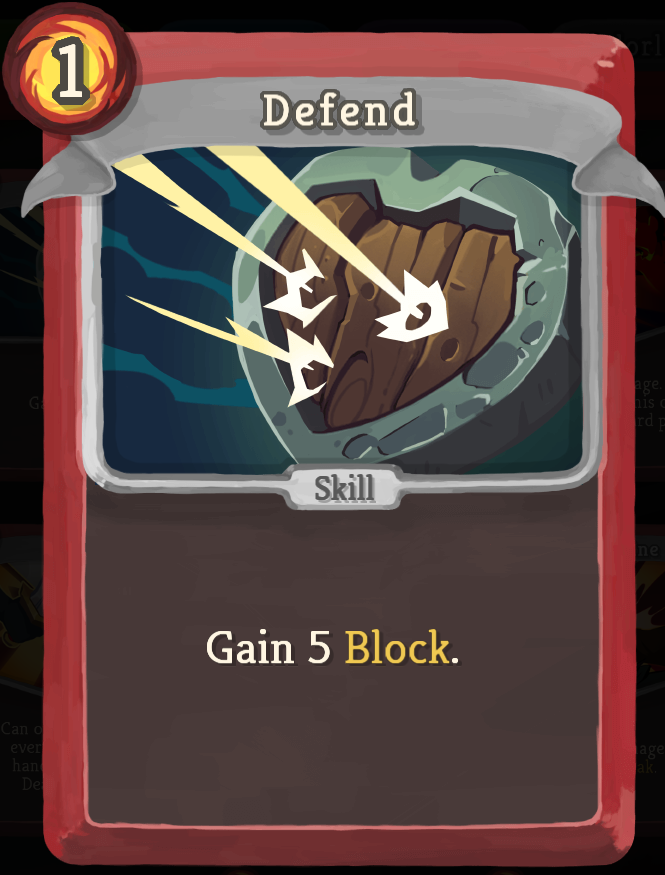
\includegraphics[width=0.95\textwidth]{img/Slay-the-Spire-Defend.png}
    \end{minipage}%
    \begin{minipage}{.25\textwidth}
        \centering
        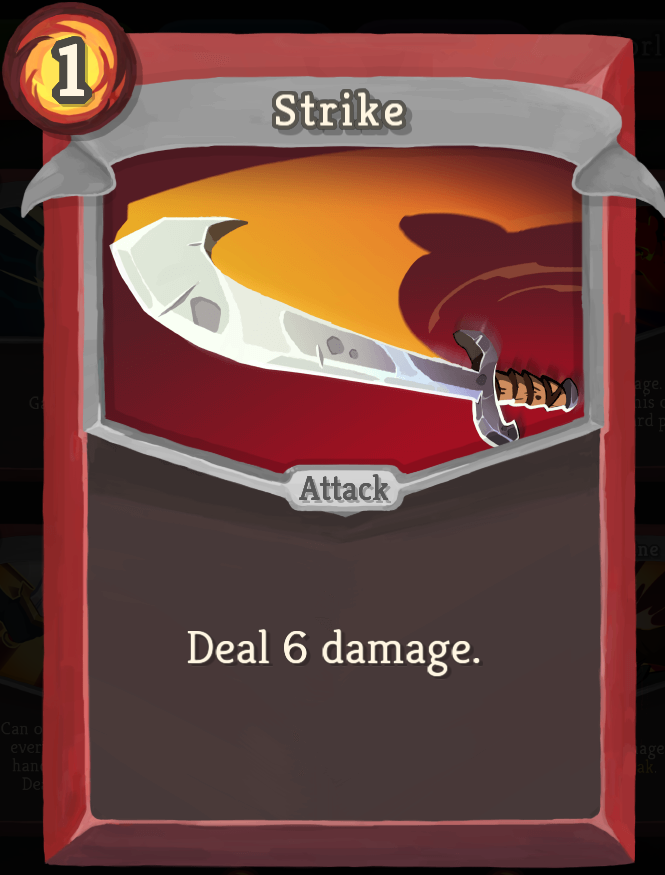
\includegraphics[width=0.95\textwidth]{img/Slay-the-Spire-Strike.png}
    \end{minipage}%
    \begin{minipage}{.25\textwidth}
        \centering
        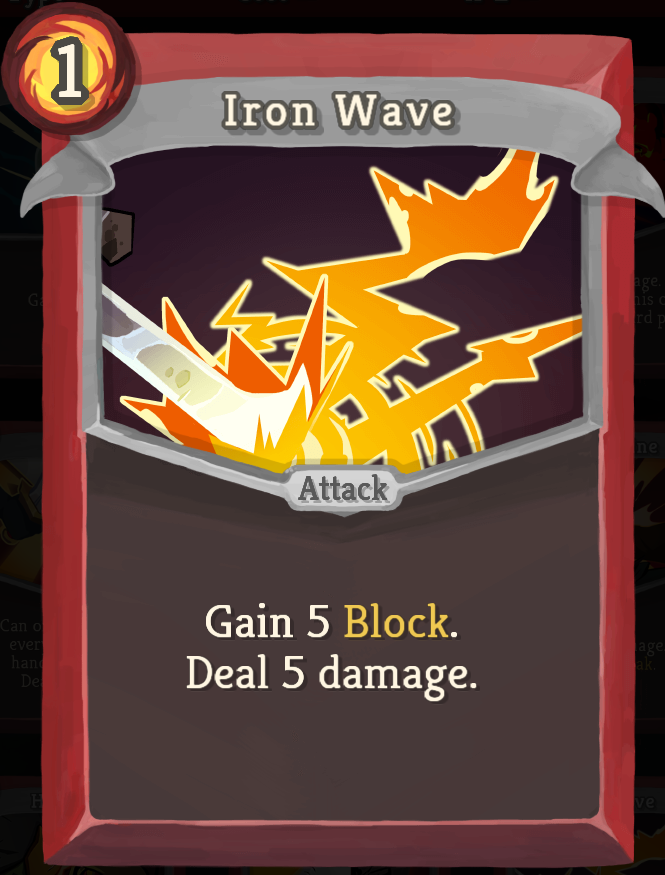
\includegraphics[width=0.95\textwidth]{img/Slay-the-Spire-Iron-Wave.png}
    \end{minipage}%
    \begin{minipage}{.25\textwidth}
        \centering
        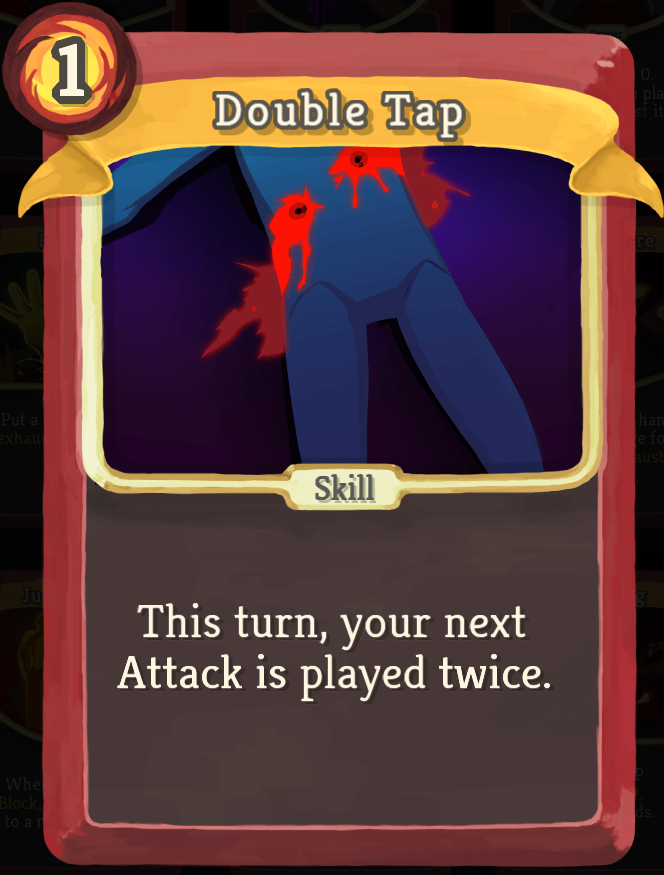
\includegraphics[width=0.95\textwidth]{img/Slay-the-Spire-Double-Tap.png}
    \end{minipage}
    \caption{\emph{Defend}, \emph{Strike}, \emph{Iron Wave} and \emph{Double Tap} cards from \emph{Slay the Spire}.}
    \label{fig:sts-iron-wave-and-double-tap}
\end{center}

We can design the blueprints in our game similarly, making some useful early in the run and some powerful later.
This will let the player decide if they need to take a blueprint that will help them now, or a blueprint that can potentially be strong later.

\subsection{Make Various Builds Viable} \label{sec:goal-various-builds}

One of the goals of our game is that the player should be able to beat the game with a lot of different combinations of blueprints.
We will call these combinations \emph{builds}, as is often done~\cite{buildDict} for unique combinations of skills, attributes and items a player's character can have in a role-playing game.
Builds are distinguished mainly by what they feel like to play with.
If two blueprints are used in the same way, then exchanging one for the other doesn't make a new build.
To allow the player to choose from various builds, there has to be enough blueprints that feel distinct and better yet, they should interact with other blueprints in unique ways.

In figure \ref{fig:pvz-almanac} are shown all the plants from \emph{Plants vs.\ Zombies}.
As we can see, there is a lot of them, and various combinations that work well are possible.
The plants usually don't interact with each other strongly, so the player mostly has to combine the plants such that they have no weak spots.
For example, longer levels require both cheap and expensive defensive plants.
The cheap plants are used at the start of the level, and later they are replaced by the more expensive ones to fit more firepower on the limited lawn.
Some plants can struggle against certain zombie types, so the player also wants to choose plants to cover for all their weaknesses.

\begin{center}
    \captionsetup{type=figure}
    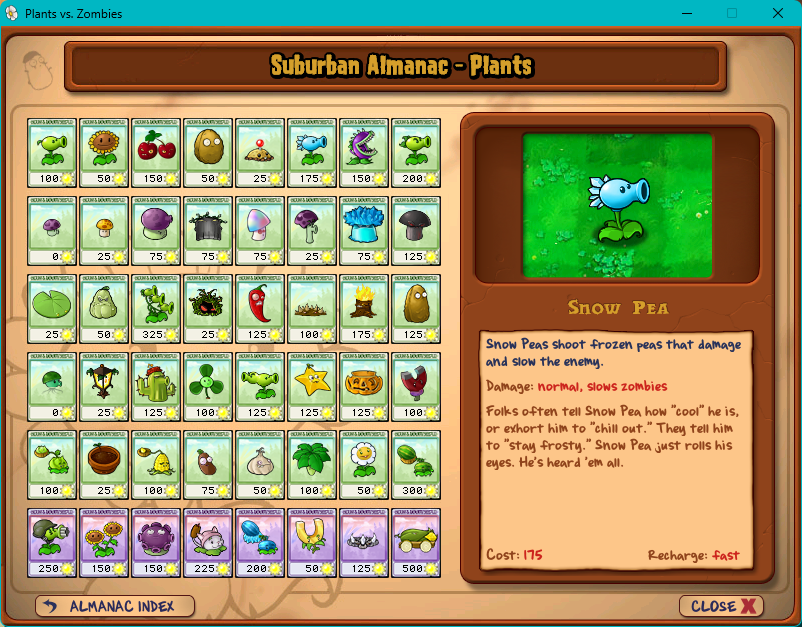
\includegraphics[width=0.8\textwidth]{img/Plants-vs-Zombies-Almanac.png}
    \caption{All the plants of \emph{Plants vs.\ Zombies} in the in-game almanac.}
    \label{fig:pvz-almanac}
\end{center}

We can also look at a few examples from \emph{Slay the Spire}.
Here, builds are often defined by cards that interact in ways that make them stronger.
One of the most blatant examples are cards that apply \emph{poison} to the enemy.
A poisoned enemy takes damage every turn based on the amount of \emph{poison} they have, and the amount decreases by one every turn.
This means an enemy with 2\,\emph{poison} takes $2 + 1 = 3$ damage in total, whereas an enemy with 4\,\emph{poison} takes $4 + 3 + 2 + 1 = 10$ damage in total.
It's easy to see that every card that applies \emph{poison} makes other \emph{poison} cards stronger.

There are also rare cards the player can find, which change how the game works.
For example, defensive cards provide \emph{block} only for one turn because the player character loses all \emph{block} at the start of every turn.
However, once the player plays the card \emph{Barricade}, they don't lose block at the start of their turns for the rest of the fight.
Cards like this can determine the player's strategy for the rest of the game on their own.

We want the players of our game to try lots of different builds and for that, the builds need to be strong enough to beat the game when the player executes them well.
We can tweak the strength of individual blueprints, but we can also design enemies that punish specific builds that would otherwise be too good.
For example, in \emph{Slay the Spire}, many enemies shuffle unplayable cards into the players deck for the duration of the fight.
This punishes decks with fewer cards way more than decks with many cards, keeping small deck builds from being too powerful.

\subsection{Force Exploration} \label{sec:goal-force-exploration}

We don't want the player to just find a single build that works and never explore anything new.
When the player is familiar with a build, it becomes stronger, since they know how to use it effectively.
This discourages them from trying other builds, because they can't use them so well, making them weaker.
Thus, one of our goals is to force the player to explore and make them learn other strategies.

The main way to get cards in \emph{Slay the Spire} are the rewards after every battle, where the player can choose one of three cards to add to their deck, as shown in figure \ref{fig:sts-card-reward}.
All the ways to acquire cards are randomized, so the player can't just hope to always get the card they want.
They have to adapt their build to the cards on offer, so they have to explore different strategies in order to win consistently.
In our game, the player will also pick a blueprint to add to their collection from a randomized offer after each battle.

\begin{center}
    \captionsetup{type=figure}
    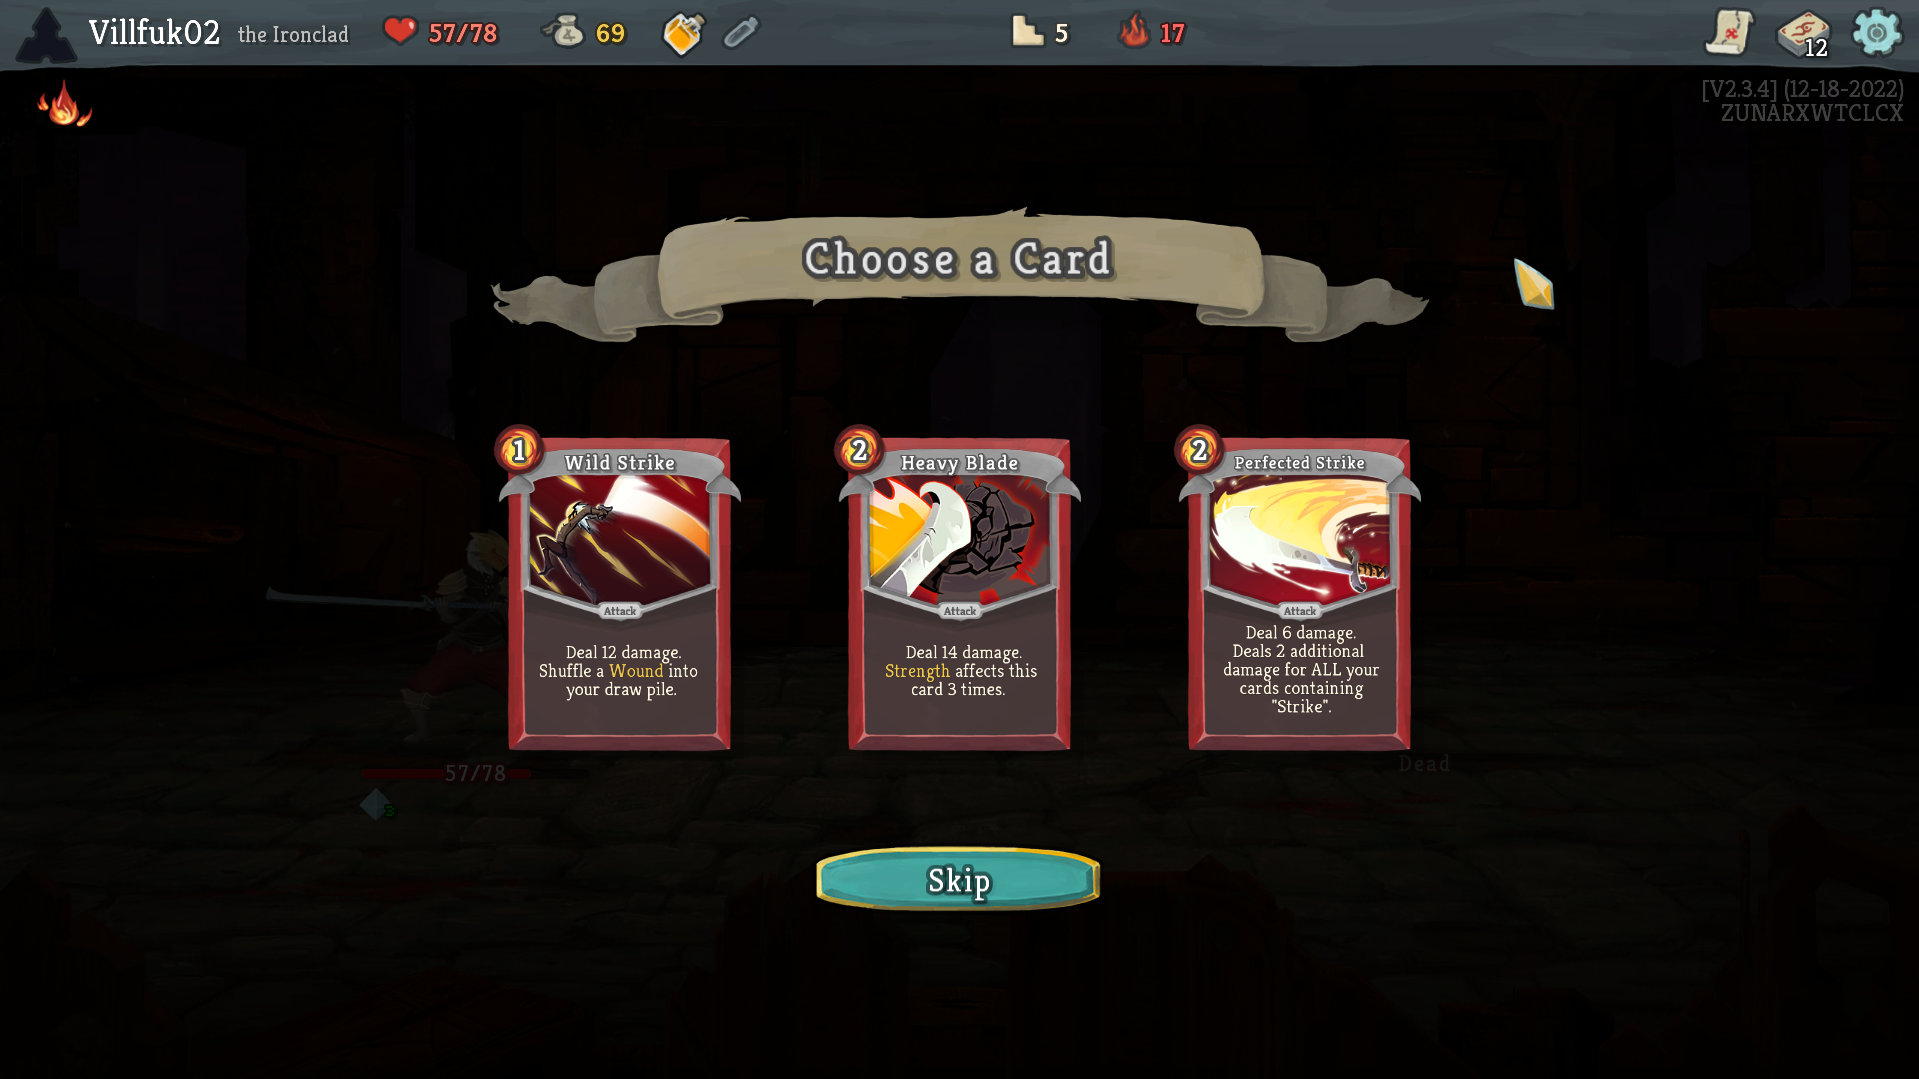
\includegraphics[width=0.8\textwidth]{img/Slay-the-Spire-Reward.png}
    \caption{Card reward screen in \emph{Slay the Spire}.}
    \label{fig:sts-card-reward}
\end{center}

In \emph{Plants vs.\ Zombies}, the player has to adapt to different zombies and level environments.
This can be illustrated with figure \ref{fig:pvz-roof}, which shows a seed select screen.
Here, the player selects which plants they want to use in this level from the selection on the left side.
On the right the player can see that this level takes place on the roof and the zombie types that will appear in this level.
In rooftop levels, the player has to place a \emph{Flower Pot}, which costs 25\,\emph{sun}, on a tile before they can place a plant there.
Furthermore, all plants that shoot in a straight line are of little use here because the roof slopes up, so their projectiles can't travel very far.
An experienced player will also notice that \emph{Bungee Zombies} will appear.
These zombies swing from above to take the player's plants instead of coming from the right.
The player should consider all these factors when choosing the build to play this level with.

\begin{center}
    \captionsetup{type=figure}
    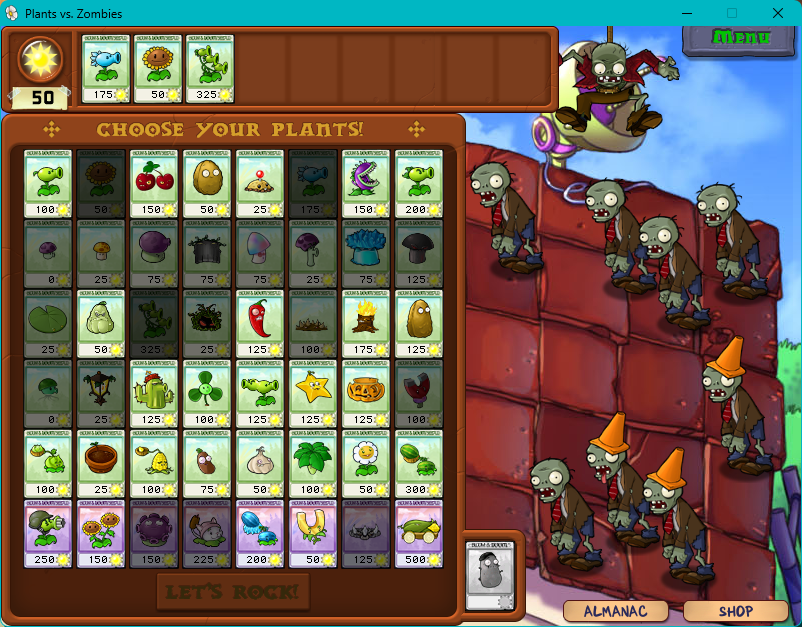
\includegraphics[width=0.8\textwidth]{img/Plants-vs-Zombies-Rooftop.png}
    \caption{Seed select screen in a rooftop level in \emph{Plants vs.\ Zombies}.}
    \label{fig:pvz-roof}
\end{center}

In our game, the player could select which blueprints to play with before every battle based on the level's features and attackers.
Instead, we chose an approach more similar to \emph{Slay the Spire}~--- the player will keep the blueprints they collect for the rest of the run, and they won't know the specifics of a battle before selecting it.
However, they will be allowed to have only a limited amount of blueprints at once, so they still cannot just keep all the blueprints they encounter.

\subsection{Provide a Challenge} \label{sec:goal-challenge}

The player should always have some goal to work towards, just out of their reach.
If the game is too easy, the players will have no reason to think strategically or learn.
Always having a harder challenge to overcome will motivate the player to improve and keep playing.

\emph{Slay the Spire} is not easy to beat, but the player can still improve so much even after beating the game.
After beating the game, the player unlocks so-called \emph{ascension}.
Before embarking on another run, the player can select the \emph{ascension} level they want to play on.
Each level introduces a small change that makes the game slightly more difficult.
Each \emph{ascension} level is unlocked only after the previous level is beaten, and each difficulty increase is small, so it doesn't discourage the player.
These changes are cumulative, so in the end it takes serious effort and luck to beat the game on \emph{ascension} level~20 even for the most skilled players.

This system is simple, yet effective, so we might as well use it too.
We will also want to balance the base game, so that most players that try are able to beat it, but it still takes some effort and several attempts, so the players feel like they've accomplished something.

\section{Procedural Generation}

- roguelike -> procedural generation

- to what degree?

- map will be random

- we want to procedurally generate levels

- terrain types

- balance levels - cannot feel unfair

- in sts, encounters are handcrafted, but picked randomly

- still has variety

- easy to balance

- generated waves

- attacker types

- hard to balance - must be described by a formula

\section{Battle}

As stated before (see section~\ref{sec:original-vision}), in our game, the player will fight in battles throughout each run, and these battles will have tower defense gameplay.
In this section, we will describe the battles in more detail and explain our decisions.

\subsection{Attacker Behavior}

In \emph{Plants vs.\ Zombies}, the zombies come continuously throughout a level, but only in small numbers.
And then there is a few marked waves in which a lot of zombies come at once.
In other games, the attackers come only in distinct waves, but the waves come right after each other based on a timer.
One example of such a game is \emph{Kingdom Rush}~\cite{kingdomRush}.
In figure~\ref{fig:kr-next-wave}, a skull icon in a circle is shown at the top of the screen with the text \enquote{INCOMING NEXT WAVE! CLICK TO CALL IT EARLY}.
The ring around the skull fills with red color over time and once it is full, the next wave of attackers comes automatically.
Both of these options make a game more action-packed.
However, we will go with a third, also often used option, where the attackers come only in waves, but there is no timer.
The player will have plenty of time to plan out their strategy, and they start the next wave of attackers when ready.
We feel this fits our game more, making it more similar to the turn-based gameplay that is often featured in roguelike games.

\begin{center}
    \captionsetup{type=figure}
    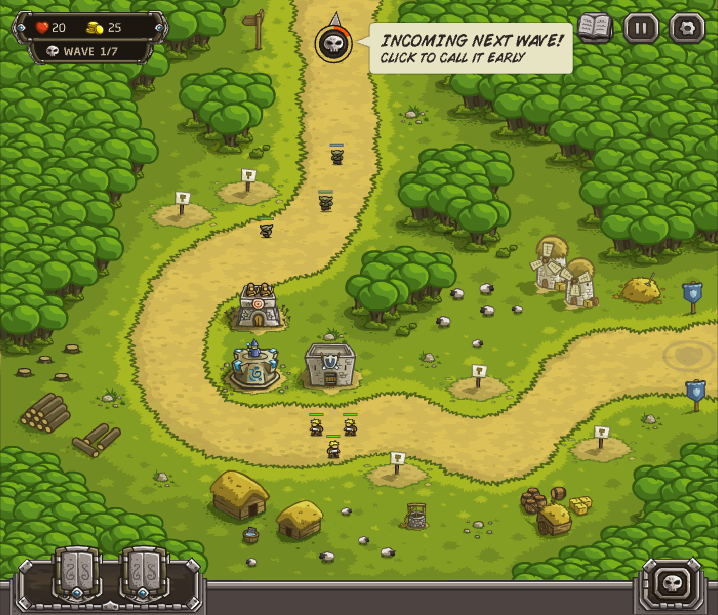
\includegraphics[width=0.8\textwidth]{img/Kingdom-Rush-Next-Wave.png}
    \caption{A screenshot from \emph{Kingdom Rush}, featuring a wave timer.}
    \label{fig:kr-next-wave}
\end{center}

Different tower defense games also use various types of attacker movement.
In \emph{Plants vs.\ Zombies}, the zombies come from the right side of the screen and try to reach the left side, as we already mentioned.
Each zombie is confined to its lane and most of the plants available to the player only affect the zombies in front of them in the same lane.
The plants are planted directly in the way of the zombies and the zombies have to eat their way through the plants to reach their goal.
This is, however very restrictive for the design of the towers in our game, and there is little depth to the tower placement.
We can let the attackers move in two dimensions to allow for more interesting tower placement decisions.

In \emph{Desktop Tower Defense}~\cite{DTDWiki}, for example, the attackers move from sides of the rectangular playing field to the sides that lie across.
The playing field starts out empty, but as the player fills it with towers, the attackers have to adjust their path, because they cannot go through the towers, as shown in figure~\ref{fig:dtd-pathfinding}.
Since the player decides the path of the attackers, they have to learn what kind of path works well, but then they can use it build it all the time.
This is not ideal for us, because we want the player to adapt to the environment, not the other way around.
Also, a path always has to exist through, so \emph{Desktop Tower Defense} doesn't let the player place a tower that would disconnect the attacker entrance from their goal.
Some games allow the player to block off the path completely, and then the attackers attack the player's towers, similarly to \emph{Plants vs.\ Zombies}.
But for our game that would be just more unnecessary complexity, since we want to focus more on the offensive abilities of the towers.

\begin{center}
    \captionsetup{type=figure}
    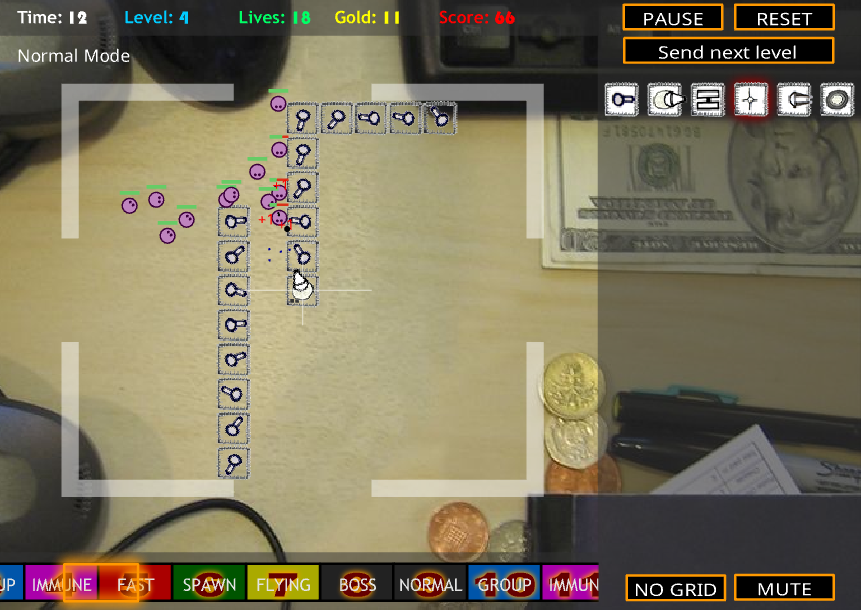
\includegraphics[width=0.8\textwidth]{img/Desktop-Tower-Defense-Pathfinding.png}
    \caption{A screenshot from \emph{Desktop Tower Defense}.}
    \label{fig:dtd-pathfinding}
\end{center}

Instead, we chose an approach that is most common in tower defense games~--- the attacker paths are predetermined, and the player builds their towers around the paths.
The paths are different in every level, so the player has to think about placement of their towers differently, and it makes different towers more useful than others in each level.
This is illustrated well on figure~\ref{fig:btd6-maps}, where we can see two levels from \emph{Bloons TD 6}~\cite{BTD6}.
The path in the first level shown has a lot of tight turns, perfect for close-range towers or towers which damage all attackers in an area.
In the second level, the path is made up of few long straight segments, where are much more useful towers, which pierce through many attackers in a straight line.

\begin{center}
    \captionsetup{type=figure}
    \begin{minipage}{.5\textwidth}
        \centering
        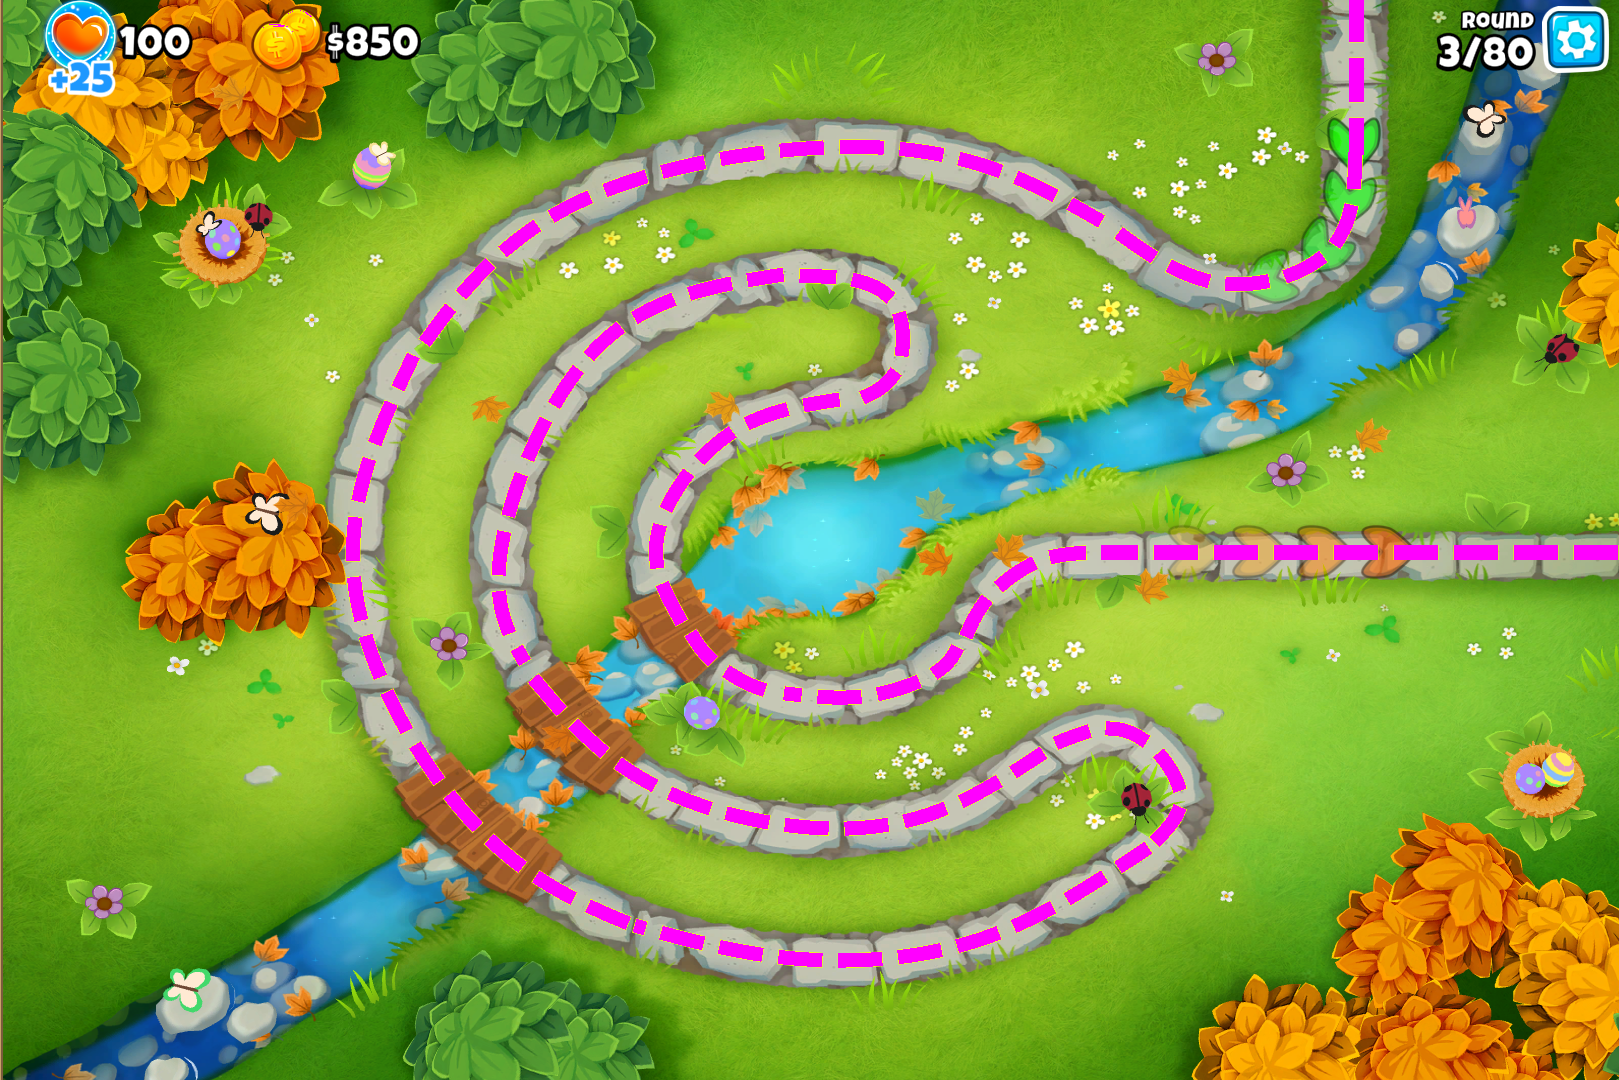
\includegraphics[width=0.95\textwidth]{img/Bloons-TD6-Park-Path-Highlighted.png}
    \end{minipage}%
    \begin{minipage}{.5\textwidth}
        \centering
        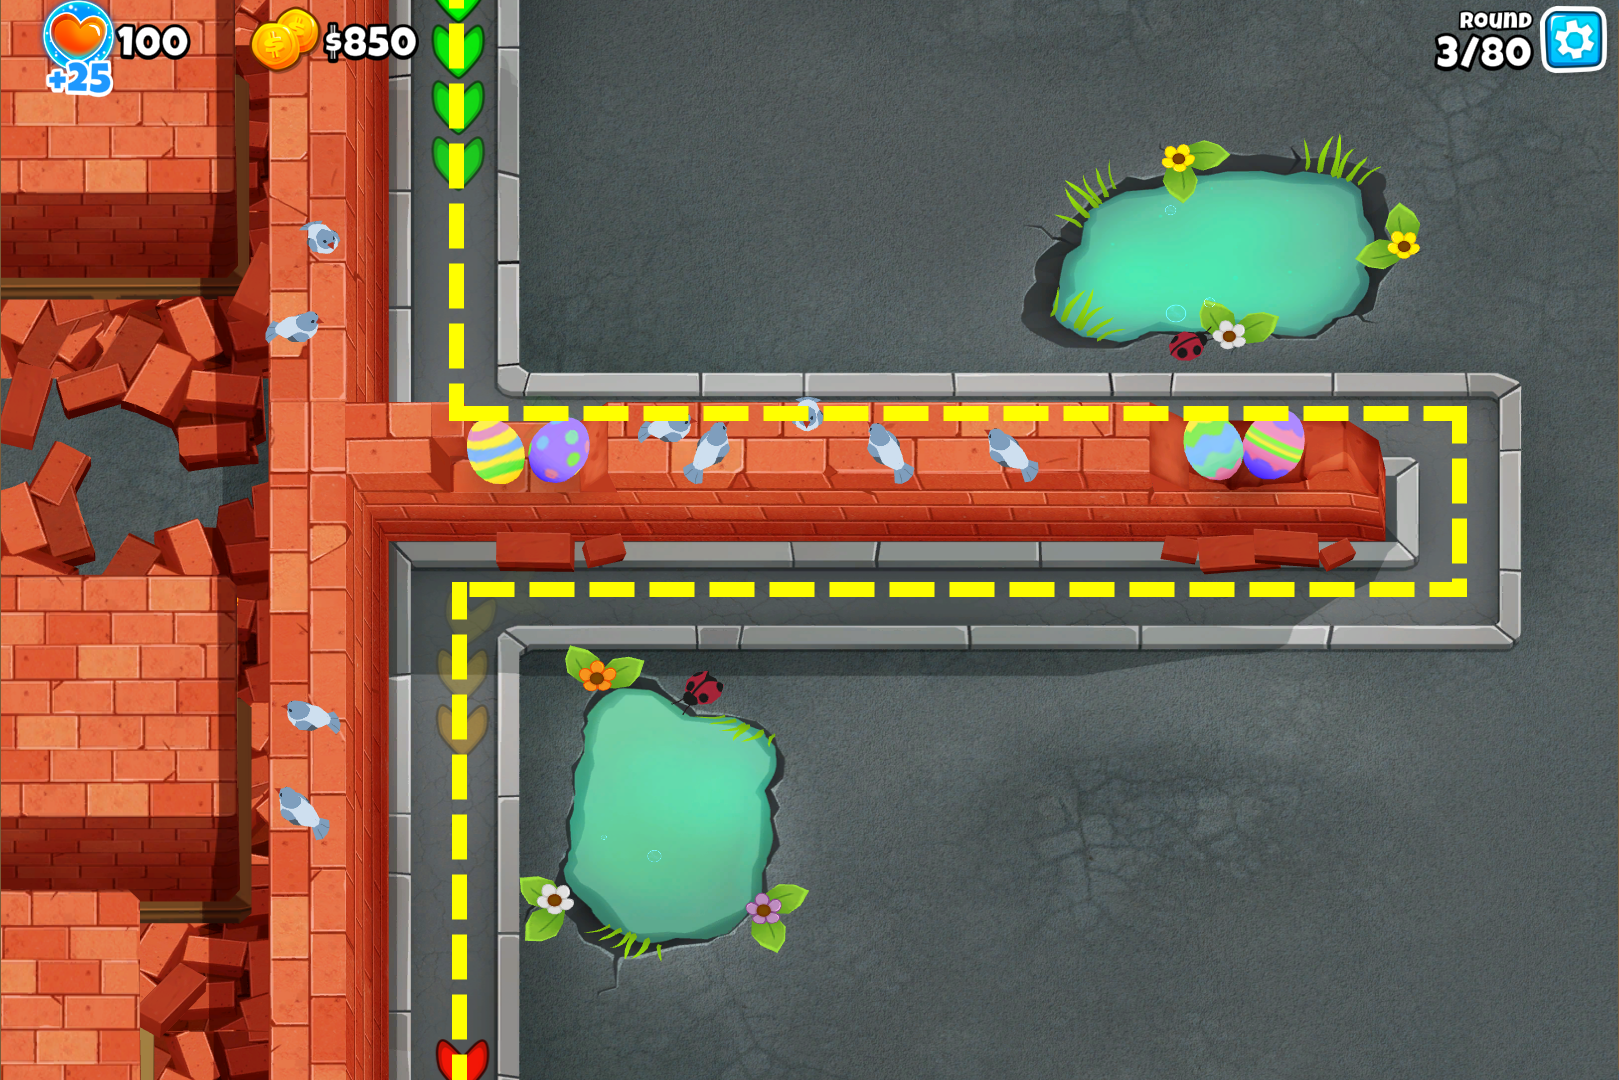
\includegraphics[width=0.95\textwidth]{img/Bloons-TD6-Another-Brick-Highlighted.png}
    \end{minipage}
    \caption{The levels \emph{Park Path} and \emph{Another Brick} from \emph{Bloons TD 6} with the attacker paths highlighted.}
    \label{fig:btd6-maps}
\end{center}

More variety can also be added by having multiple paths in a single level.
We can even have different attackers on each path in some waves to further increase variety.
The paths in our game will also be able to split into more paths and join together into one path.
When a line of attackers comes to a split into multiple paths, they will alternate in which path they continue to, splitting between the paths evenly.
This creates segments with lower attacker density, which makes certain towers less effective around this part of the path.
On the other hand, this lets the player fit more towers near these two paths than they could fit around the path if it didn't split.

\subsection{Attacker Paths}

If we designed each level of our game by hand, we could create paths that just feel like they would be fun to play around.
Since the paths will also be procedurally generated, we need to describe what qualities should the paths have, so the generation can later be implemented to produce such paths.
For reasons that will be explained in the next subsection, the paths and towers will be confined to a square grid of tiles.
Let's start with a few basic rules:
\begin{itemize}
    \item A level can have one or more paths, and paths can split apart or join together.
    \item Each path will be composed of segments that go from the center of one tile to the center of an orthogonally adjacent one.
    \item The paths will start just outside the world and end at the tile with the \emph{Hub}.
\end{itemize}
In figure~\ref{fig:valid-path-example} we can see an example of a valid path drawn in blue on a backdrop of the square tiles the world is composed of.
The \emph{Hub} is represented by a black dot.

\begin{center}
    \captionsetup{type=figure}
    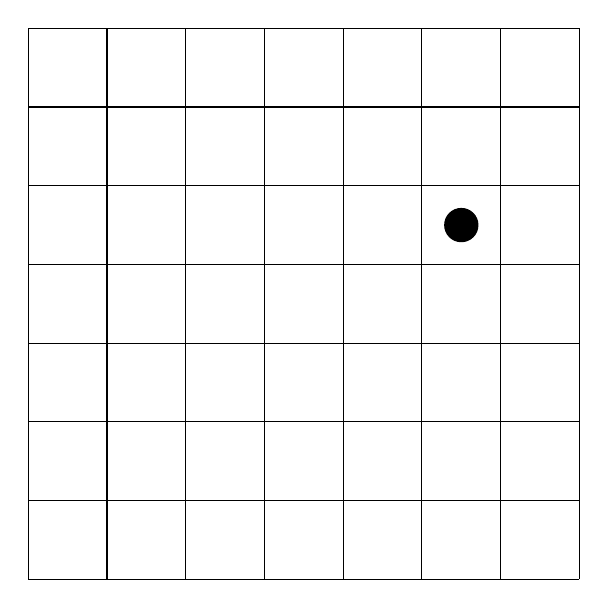
\begin{tikzpicture}
        \draw[step=1.0,black,thin] (0,0) grid (7,7);
        \drawpath{-1,1}{right}{}{(3,1)--(3,2)--(1,2)--(1,5)--(3,5)--(3,4)--(5,4)}{0.5}
        \filldraw[black] (5.5,4.5) circle (6pt);
    \end{tikzpicture}
    \caption{An example of a valid path in the game world.}
    \label{fig:valid-path-example}
\end{center}

However, we need more rules, since right now, nothing forbids a path going back on itself.
This is illustrated with path \textbf{A} in figure~\ref{fig:ambiguous-paths}, where we offset the endpoints of few segments to make it more readable.
Paths segments have to start and end in the centers of the tiles, so in reality, it would look like path \textbf{B}, which is definitely unreadable.

Furthermore, no path should cross itself or another path.
We want this because the paths can split and join, and we would need a way to distinguish these splits and joins from crossings.
This is done to make sure the paths are readable to the player.
For example, the paths \textbf{C} and \textbf{D} in figure~\ref{fig:ambiguous-paths} could very much be crossing each other, but they could also join together and split in two on the same tile.
Furthermore, path \textbf{E} is ambiguous, because it could cross itself, but it also looks almost as if it split and joined with itself on the same tile.

\begin{center}
    \captionsetup{type=figure}
    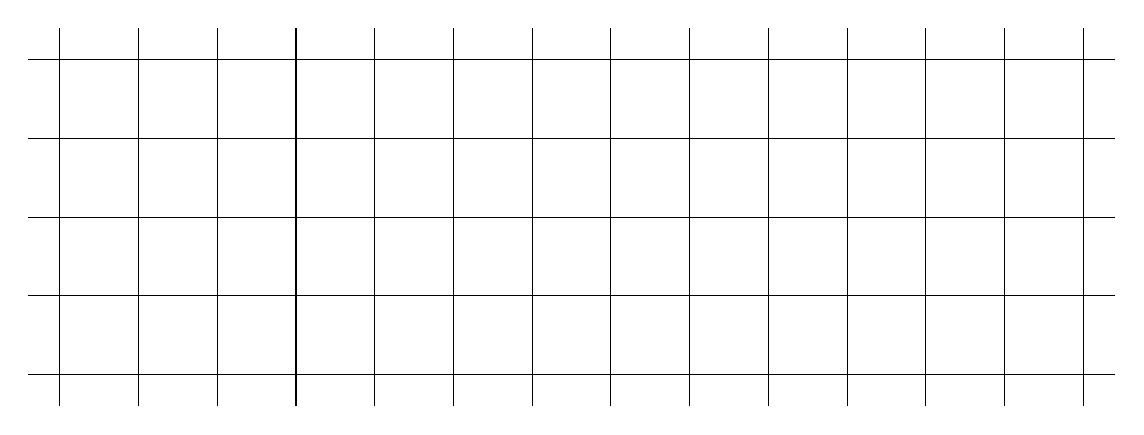
\begin{tikzpicture}
        \draw[step=1.0,black,thin] (0.6,0.6) grid (14.4,5.4);
        \drawpath{1,5}{above}{A}{(1.2,2)--(0.8,3)--(1,0)}{0.51}
        \drawpath{3,5}{above}{B}{(3,2)--(3,3)--(3,0)}{0.5}
        \drawpath{5,5}{above}{C}{(5,3)--(8,3)--(8,0)}{0.5}
        \drawpath{7,5}{above}{D}{(7,0)}{0.5}
        \drawpath{12,5}{above}{E}{(12,1)--(10,1)--(10,3)--(14,3)}{0.5}
    \end{tikzpicture}
    \caption{Several paths that would be confusing or ambiguous if paths could cross.}
    \label{fig:ambiguous-paths}
\end{center}

Path \textbf{F} in figure~\ref{fig:distance-to-hub-paths} is however also problematic.
It does not cross over itself, but if we were to center all the segment endpoints, it would look almost like path \textbf{E}, which would be equally confusing.
We will redefine make no-crossing rule stronger and define it as the following:
\begin{itemize}
    \item Each path segment makes a one-way connection from a tile to its neighbor.
          The distance of each tile connected to the \emph{Hub} must be the same, no matter which path an attacker takes.
\end{itemize}
This makes path \textbf{F} also illegal, since it goes through a tile twice, and the second time it visits it, it is 8 segments closer to the \emph{Hub} than before.
This also has implications for paths that split or join, for example path \textbf{G} is invalid, as demonstrated by the distances shown in red, while the path network \textbf{H, I} is valid.
The new rule helps here, because we don't want the spacing between attackers to change only because some took a longer path before merging with the attackers that took a shorter path.

\begin{center}
    \captionsetup{type=figure}
    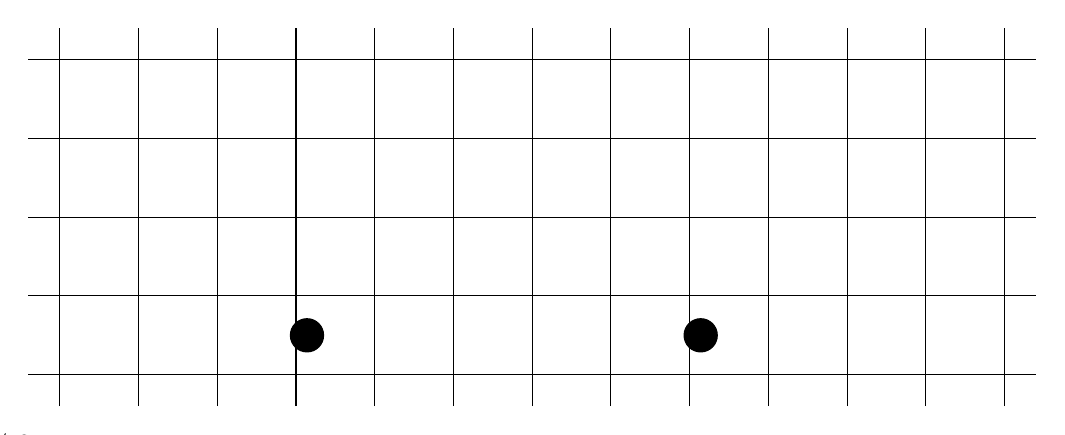
\begin{tikzpicture}
        \draw[step=1.0,black,thin] (1.6,0.6) grid (14.4,5.4);
        \drawpath{12,5}{above}{F}{(11.9,3.1)--(10,3)--(10,1)--(12,1)--(12.1,2.9)--(14,3)}{0.485}
        \drawpath{8,5}{above}{G}{(8,4) node[red]{$5 \neq 3$} --(8,3) --(8,2) node[red,right]{1} --(8,1)}{0.5}
        \drawpath{8,3}{above,red}{$4 \neq 2$}{(7,3) node[left,red]{3}-- (7,2) node[left,red]{2}-- (8,2)}{0.5}
        \filldraw[black] (8.5,1.5) circle (6pt);
        \drawpath{5,5}{above}{H}{(5,4) node[right,red]{5} -- (5,3) node[right,red]{4} -- (5,2) node[right,red]{3} -- (5,1) node[below right,red]{2} -- (4,1) node[below,red]{1} --(3,1)}{0.5}
        \drawpath{2,5}{above}{I}{(2,4) node[left,red]{4} -- (2,3) node[left,red]{3} -- (3,3) -- (3,2) node[left,red]{1} --(3,1)}{0.5}
        \drawpath{5,3}{}{}{(4,3) node[above,red]{3} -- (3,3) node[above,red]{2}}{0.5}
        \filldraw[black] (3.5,1.5) circle (6pt);
    \end{tikzpicture}
    \caption{Several paths illustrating the rule that each tile can only have one distance to the \emph{Hub}.}
    \label{fig:distance-to-hub-paths}
\end{center}


- paths near each other are undesirable

- tight turns are undesirable

- short splits are banned

- fill the world as much as possible

\subsection{World}

- grid of tiles \checkmark

- more granularity, easier to develop intuition, same for attacker paths

- free placement X

- preset places

- 3D \checkmark
- Simple and intuitive way to make the level itself more interesting
Some towers won't be able to shoot uphill or downhill - more interesting decisions for the player

- Terrain types (for now, just one)

- Obstacles

\subsection{Buildings}

- how and when to build, one per tile
- only between waves

- special building have special abilities

- main types:


\subsection{Towers}

- attack attackers

- range

- targeting

- projectile types

- damage types

\subsection{Economic buildings}

-provide resources

- materials - what, why, consequences and constraints

- fuel?

\subsection{Abilities}

- used mid-wave

- usually instant effects

- free placement, global placement, tile placement, use on a building

- energy - what, why, consequences and constraints


\section{Battle Graphical User Interface}

\xxx{specify controls, use images}

\subsection{Waves Left and Fuel}

\subsection{Hull}

\subsection{Wave Preview}

\subsection{Materials and Energy}

\subsection{Blueprints}

- what they represent

- limited number

- cost and cooldowns

- rarities

- make them unique

- lenticular design

\subsection{Info Panel and Selection}

- what it looks like and what's on it

- select blueprints

- select buildings

- select attackers

\subsection{Highlights and Range Visualization}

\section{Attackers}

- move, have health

- sizes

- special abilities - passive, repeating, reactive

\section{Camera controls}

- zoom to look closely, rotate so the terrain doesn't hide stuff

\section{Future Features}

- setting

- run structure

- map

- events and shops

- saving the game

- unlocks

- difficulty levels
